% !Mode:: "TeX:UTF-8"
\chapter{限制分支预测宽度的改进策略}

本章首先介绍香山第一版架构的取指策略,为什么需要限制分支预测的宽度,过宽的分支预测宽度会对整体设计带来怎样的影响。之后介绍如何通过修改每拍取指的基本单位来限制同一次取指内容中分支指令和跳转指令上限。

\section{香山第一版取指策略}

在香山第一版的设计中,取指pc是按照32Bytes对齐的,也就是低5位都为0,然后每次取指固定取32Bytes的指令数据。由于实现了RISC-V的C扩展,即压缩指令集,RISC-V正常的一条指令 (RVI) 占4个Bytes,而C扩展中规定了许多压缩指令 (RVC),这些压缩指令只有2个Bytes长。

增加了压缩指令之后,会带来一些问题,首先就是分支指令可能会跨行,如图3.1所示,为了便于表示,以一个cache line 8Bytes为例,当然实际设计中一个cache line会大得多。图3.1(a)是不带压缩指令的情况,所有指令都是对齐的,不会出现一条指令在两个cache line中各存一半的现象,但是加入了压缩指令之后就会出现图3.1(b)的这种情况,即由于加入了压缩指令,非压缩的指令无法对齐,就会出现一条非压缩指令被2个相邻的cache line截断的情况。

当出现这种情况时,就会导致最后这条分支指令无法在一个周期内被完整取出,如果这条被截断的指令正好是条分支,也只有等到下一周期取到后半条指令码后才能对它进行预译码操作。

\begin{figure}[htb]
    \centering
    \setlength\tabcolsep{3pt}  % 同一行中的图片间隔
    \vspace{5pt} % 图片上部的空白,如果太小的话,图片顶部会与正文内容十分接近
    \begin{tabular}{ccc}
        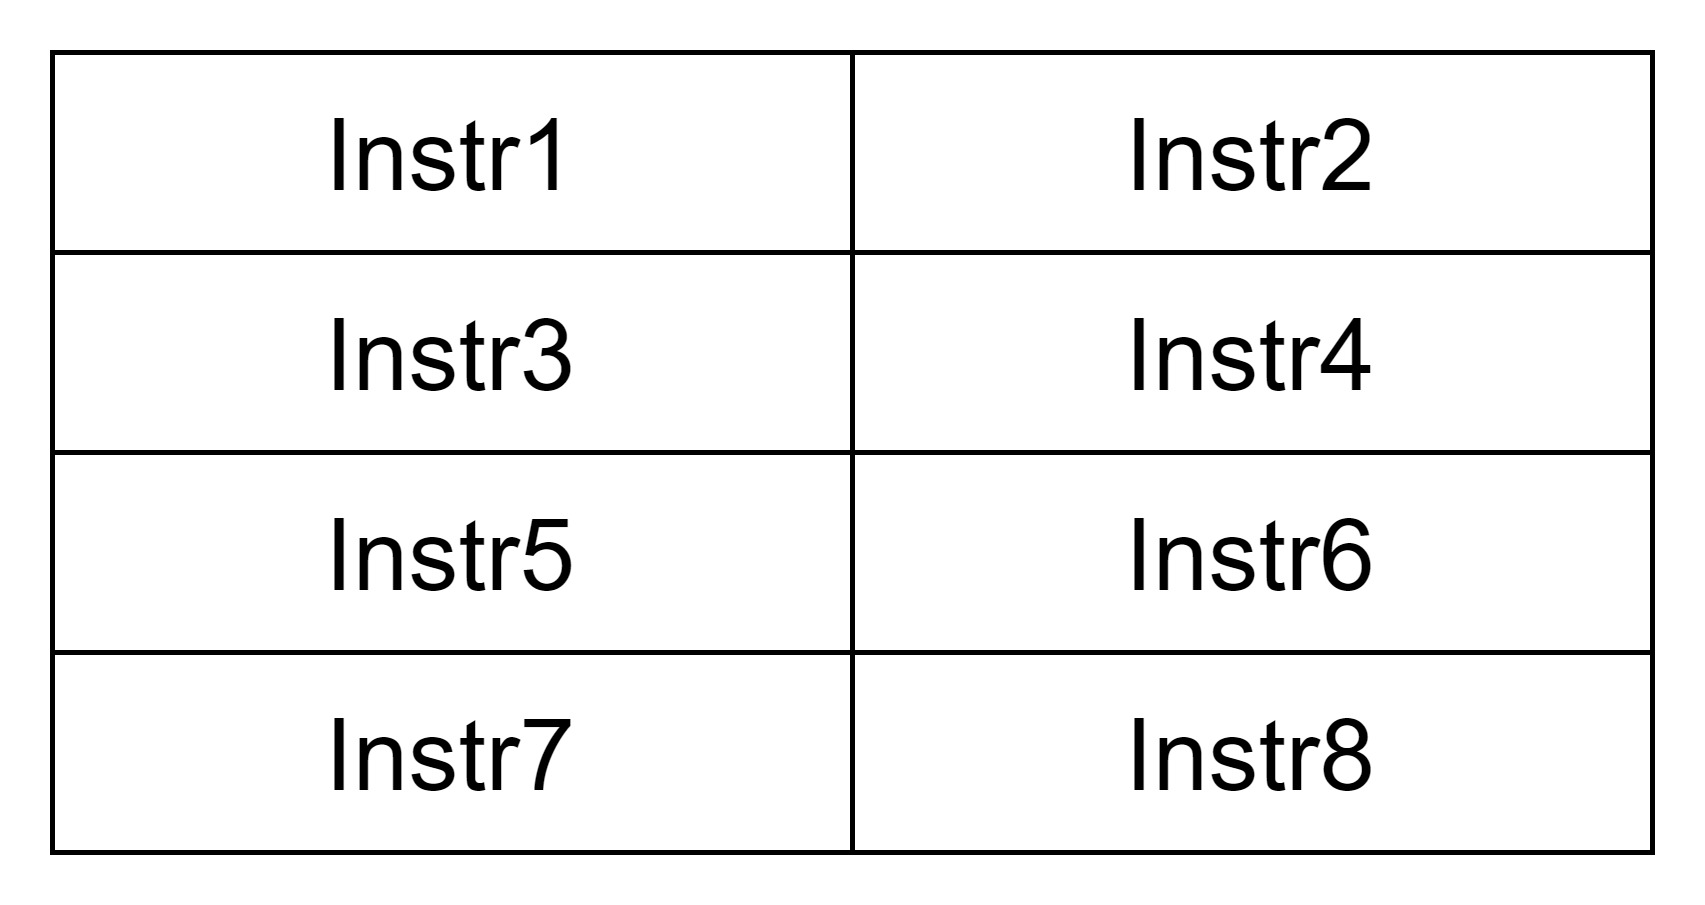
\includegraphics[width=0.30\textwidth]{RVI-only.jpg} &
        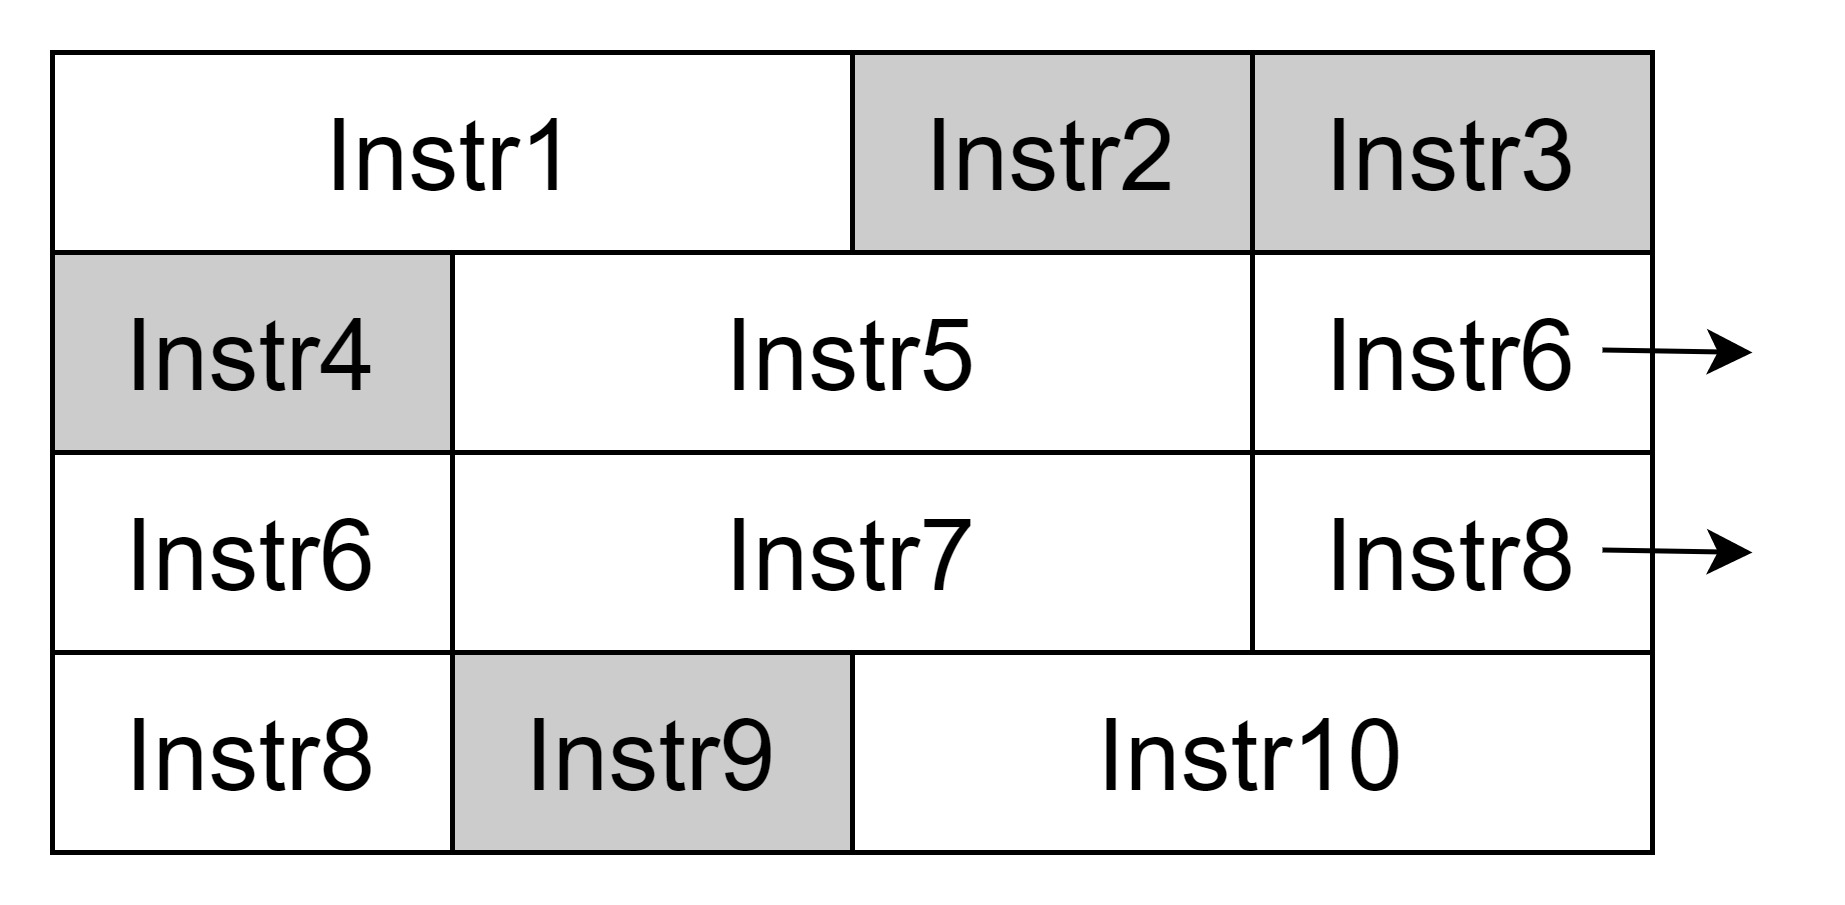
\includegraphics[width=0.325\textwidth]{RVIC.jpg} &
        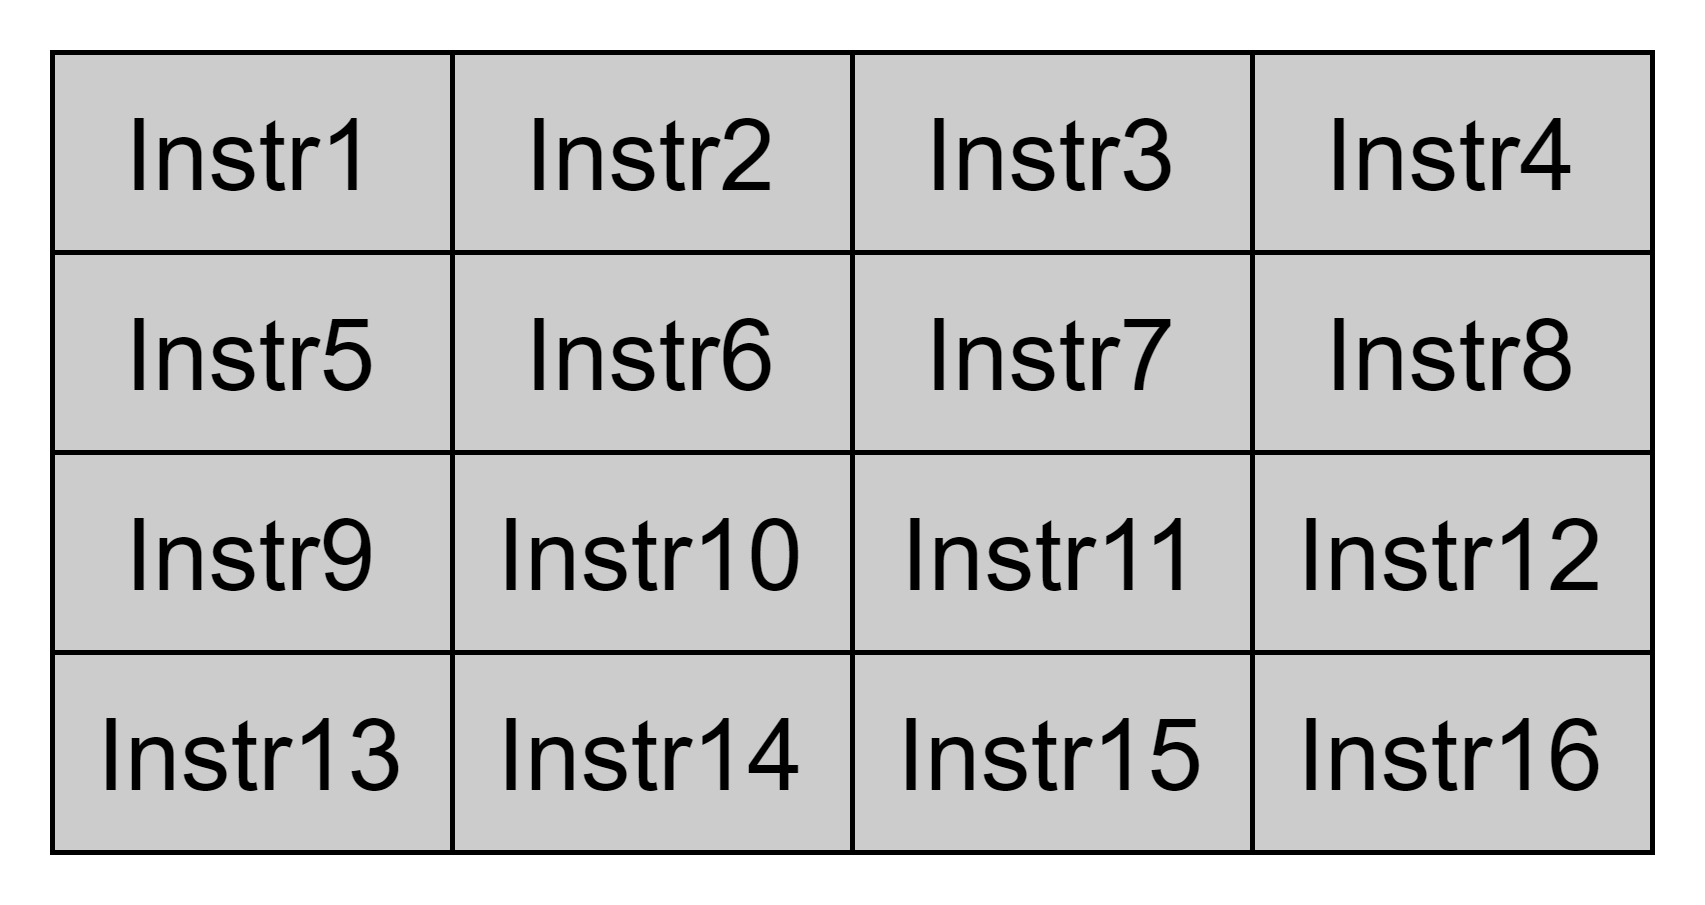
\includegraphics[width=0.30\textwidth]{RVC-only.jpg} \\
        (a) 只有RVI指令 & (b) RVI,RVC指令混合 & (c) 只有RVC指令 \\[1ex]
    \end{tabular}
    \caption{在cache line中以不同形式储存的指令码,其中白色的代表非压缩指令RVI,灰色的代表压缩指令RVC,图(b)中第6和第8条指令跨cache line了}
    \label{fig:figure1}
\end{figure}

加入了压缩指令之后,如果以32Byte为单位取指,每次取出来的数据中会有8到16条指令不等,最多的情况如图3.1(c)所示,即16条都是压缩指令的情况。因此为了能够覆盖到所有情况,香山第一版的分支预测设计中,所有的预测器,包括第一版中FTB的原型BTB (Branch Barget Buffer) 都是以16为宽度来设计的,也就是说每个预测器都有16个bank,每个bank对应32Bytes中所有有可能是一条分支的位置。

但是实际上真正在程序运行中一次取指有这么多条分支的情况非常少见,这种设计在一定程度上是冗余的,这种设计意味着所有的分支预测逻辑的复杂度和连线都会大大增加,尤其是在分支预测最终的时候,我们需要从所有的分支中选出一条最终预测跳转的分支,从16个备选项中选出目标跳转地址,这是一个4级的多选操作,而这个逻辑处于分支预测的很多路径上,是关键路径的一部分,因此降低分支预测宽度,能够减少分支预测的逻辑复杂度,减少最终选择需要的逻辑门数,最终达到优化时序,提高频率的效果。

\section{Fetch Block的定义}

为了降低分支预测宽度,我们需要限制每次取指所能包含的分支指令的最大数量,因为分支预测最终的宽度是以可能的最大分支数量为准的,例如上文提到的如果一次最多会有16条分支,那么分支预测宽度也必须为16,即使大部分时候并没有这么多分支。
假设我们将分支预测的宽度限制为2,之前的取指是以32Byte定长为单位取指的,而在一些分支指令密集的程序片段中,32Bytes大小的指令块中很大概率会出现超过2条分支,因此我们不能够继续以固定的大小作为取指的基本单位,我们需要定义一个新的基本单位,为这个单位添加一些约束条件,以此来限制每次取指的分支指令数量。

我们定义了Fetch Block,这个概念是在Glenn的论文中提出的,每个Fetch Block都必须遵守以下的约束:

\begin{enumerate}
    \item 每个block的最大大小为32Byte
    \item 当遇到第n+1条条件跳转指令 (branch) 时,无论block大小有没有32Byte,这个block都在第n+1条条件跳转指令之前截止
    \item 当遇到无条件跳转指令 (jump) 时,无论block大小有没有32Byte或有没有达到n条条件跳转指令的上限,这个block都在这条jump指令后截止。
\end{enumerate}

通过以上的3条约束,我们就能够保证单个的Fetch Block中branch和jump指令数量的上限。

而在此基础上,我们提出了一种改进策略,可以略微减少FTB表项的大小,节省一些面积。我们观察到,因为遇到第n+1条指令导致block截止时,其中存储jump的slot被闲置了;而遇到jump,且之前不足n条branch时,第n条branch的slot也被闲置了,而这两种情况非常常见,带来了空间的浪费。我们针对这种现象做出了改进,即令第n条branch与jump共用一个slot,这样一个block中最多可以同时有n条branch,或者同时有n-1条branch和1条jump。

\section{FTB的数据结构设计}

% 投稿论文的主要内容

为了在硬件中实现以Fetch Block为表项的FTB,我们提出了一种FTB表项的数据结构,相关的属性以及作用在表\ref{tb:table1}中列出。通过这些属性,就能够清楚的描述一个Fetch Block的状态,以及其中含有的分支指令的相关信息。

\begin{table}[]
	\caption{FTB表项属性列表}
	\label{tb:table1}
	\centering
	\begin{tabular}{|c|c|c|}
		\hline
		属性名   & 数据类型   & 含义及作用   \\ \hline
		valid & Bool & 代表这个表项是否有效 \\ \hline
		tag & UInt & Fetch Block起始地址的高位 \\ \hline
		brSlots & Vec(FtbSlot) & 用来存储branch指令的信息 \\ \hline
		tailSLot & FtbSlot & 用来存储branch/jump指令的信息 \\ \hline
		pftAddr & UInt & \tabincell{c}{代表这个block最后一条指令的下一条指令的起始pc, \\ 存储低位,使用拼位计算} \\ \hline
		carry & Bool & 代表拼位计算时高位要不要加1 \\ \hline
		isCall & Bool & 如果block中有jump时,代表这条jump是否是call指令 \\ \hline
		isRet & Bool & 如果block中有jump时,代表这条jump是否是ret指令 \\ \hline
		isJalr & Bool & 如果block中有jump时,代表这条jump是否是jalr指令 \\ \hline
		last\_may\_be\_rvi\_call & Bool & 最后一条指令可能是半条RVI Call指令 \\ \hline
		always\_taken & Vec(Bool) & 这条指令是否总是跳转 \\ \hline
	\end{tabular}
\end{table}

其中的brSLots和tailSlot是用来存储block中的branch和jump指令信息的,它们是同一种数据结构FtbSlot,FtbSlot的相关属性以及作用在表\ref{tb:table2}中列出。

\begin{table}[]
	\caption{FtbSlot属性列表}
	\label{tb:table2}
	\centering
	\begin{tabular}{|c|c|c|}
		\hline
		属性名   & 数据类型   & 含义及作用   \\ \hline
		valid & Bool & 这条branch/jump是否有效 \\ \hline
		offset & UInt & 这条branch/jump在block中的offset \\ \hline
		lower & UInt & \tabincell{c}{这条branch/jump的target的低位, \\ branch和jump的offset length是不同的} \\ \hline
		tarStat & UInt & \tabincell{c}{这条branch/jump的高位是需要加1或者减1或者不变, \\ 0代表不变,1代表加1,2代表减1} \\ \hline
		sharing & Bool & 这个slot现在存的是一个branch还是一个jump \\ \hline
	\end{tabular}
\end{table}

一个Fetch Block的起始地址就是block中第一条指令的pc,而block的结束地址应该是block中最后一条指令的下一条指令的pc。这是由于指令分为4Byte的RVI指令和2Byte的RVC指令,所以如果存储block中最后一条指令,我们并不知道最后一条指令的长度是4Byte还是2Byte,就无法推断出这个Fetch Block后面的Fetch Block的起始地址,因此我们需要存储下一个顺序Fetch Block的起始地址,我们称为fallthrough address。而完整的fallthrough address可以通过起始地址和pftAddr (partial fallthrough address) 以及carry属性计算得到。由于一个Fetch Block最大的大小不超过32Byte,因此通常来说一个Fetch Block的起始地址和结束地址的高34位要么是相同的,要么结束地址的高34位是起始地址的高34位加1。因此我们没有必要存储完整的fallthrough address,我们只需要存储fallthrough address的低5位,以及它的高位是否需要由起始地址加1得到即可,在计算fallthrough address时只需要使用block起始地址的高34位+ carry,再与pftAddr拼接,即可得到39位的完整fallthrough address。

而FtbSlot中的lower和tarStat类似于pftAddr和carry,不同之处在于分支指令的跳转距离不止32Byte,因此lower的位数等于指令码中用于计算偏移地址的offset字段的位数。同时由于分支指令既可以向前跳转,又可以向后跳转,因此分支指令的跳转目标地址高位有3种可能:与block的起始地址相同、起始地址加1、起始地址减1。所以tarStat需要2bit位宽,可以表示0、1、-1三种情况。需要计算某条分支的跳转目标地址时,也是将起始地址的高位加上tarStat,再与lower拼接得到完整的目标地址。

isCall和isRet属性主要用于标记哪些分支需要使用RAS进行预测。isJalr用于标记哪些分支是间接跳转分支指令,需要使用ITTAGE预测器预测。

always\_taken是对于一些固定跳转分支的优化,一条分支只有在至少一次跳转之后,才会被认作有效的分支加入FTB中,而一条刚加入FTB的分支我们会为它标记为always taken,之后无论预测器预测结果如何,都会预测这条分支是跳转的,如果这条分支之后有一次不跳转,always taken标志就会被消除。

\section{FTB的管理策略}

在第一版架构BTB设计中,每次有指令提交后,会在BTB中找到本身pc对应的表项,选择空闲的way写入,如果所有的way都已经被占用,就使用随机替换方式,替换已有的一个表项。而由于在第二版的架构中我们使用了以Fetch Block为基本单位的FTB,并且我们计划将其替换策略更改为plru算法,因此FTB的管理策略有较大的改动。

在FTB的设计中,由于限制了每个Fetch Block中分支指令的最大数量,因此大部分时候一个block中的有效数据是小于32Byte的,这一定程度上会导致FTB的存储空间使用效率不高。所以,为了尽可能增大每个Fetch Block中有效指令的数量,将所有未跳转过的分支指令都看作普通的指令,只有跳转过的分支才会被记录到FTB中,这就导致了每个fetch block的大小,分支指令的分布情况,在程序执行过程中是动态改变的,因此需要有一个完善的策略,针对不同的情况对FTB中的表项进行维护。

经过分析可以将FTB表项的更新分为以下几种情况:

\begin{enumerate}
	\item 在最开始时,FTB为空,因此所有的分支指令都识别不出来,默认都是不跳转,所以最初的所有Fetch Block都是32Byte,且其中视为没有任何分支
	\item 在一次指令提交中,原有的block中检测到了新的branch,而block中的branch指令数量没有达到上限,还有多余的slot时,将新的branch插入到这个block中
	\item 在一次指令提交中,有新的branch指令加入,但block中已经没有多余的slot时,需要对比新的branch指令和block中已有branch指令的先后关系,取前n条分支按顺序加入到block中,n代表当前block中所能够存储的branch指令的最大值。剩余的一条branch需要从block中去除
	\item jump指令不存在不跳转的情况,因此一定是在新建block的时候加入到存放jump的slot中,而如果是共享slot的话,如果有新的branch,它的pc在jump指令之前,就需要将jump挤出该block,branch存入共享的slot中,这条jump指令之后会被加入到一个新建的block中
\end{enumerate}

% 这里的逻辑有空再理一理

无论是上面的哪一种情况,除了需要根据不同的情况调整slot中的数据,由于最后一条分支可能会改变,因此我们还需要修改block的fallthrough address。首先需要看这条新的branch指令能否插入到block中,如果不能,说明所有的slot都满了,且它们的指令序都在这条新的branch之前,所以根据Fetch Block的定义,block在第n+1条条件跳转指令之前截止,我们需要将fallthrough address修改为这条新的branch指令的pc。而如果这条branch指令能够插入,且新的branch是block中所有分支指令的最后一条,则将fallthrough address设为正常的起始地址加32Byte。如果不是最后一条,如果没有分支指令被替换出block,则fallthrough address不变,如果有,则将fallthrough address设为被替换出block的指令的pc。

除了维护已有的Fetch Block,如果有新的block需要写入FTB,但是对应的way已经满了,就需要选择其中一个block替换出去,在第一版的架构中BTB使用的是随机替换策略,在第二版中我们改为了PLRU替换策略,并且使用的是用Chisel实现的通用替换策略模块,可以非常快速灵活的更改替换策略。

在写入新的block时需要注意,如果这个block已经在FTB中存在了,那么我们只需要更新其中的block即可,而不能够写入两个起始地址相同的block,这样会导致查找FTB时出现多路命中 (multiple hit) 的错误,这会影响到FTB中存储信息的正确性,从而影响分支预测的性能。因此,在添加或者替换block之前,我们首先需要查找一次FTB,得知block是否已经存在于FTB中,但是由于FTB是使用单口SRAM来存储主要数据的,一拍内只能够读或者写,因此在添加或替换FTB时,首先需要阻塞分支预测流水线,因为预测也要读FTB来获取分支信息,然后花一个周期先读FTB,检查block是否已经在FTB中,下一周期再写入FTB,因此,每次添加或替换FTB时,预测流水线都会堵塞两个时钟周期。这会导致预测效率的降低,为此我们做了以下几点优化,能够减少大部分指令提交时的FTB读需求:

\begin{enumerate}
	\item 在预测时会将当前预测的block是否在FTB中命中,以及哪一way命中的信息,保存传入FTQ中,而在这个block中的指令提交时,FTQ会将这个hit信号传回FTB,如果在预测时这个block就已经存在于FTB中了,那么在指令提交时这个block大概率仍然存在于FTB中,这种情况下我们只要直接将更新后的block写入预测时保存的那个way中即可,不用再查找一次FTB。当然如果没有命中,我们仍然还是要查找一次FTB。不过通常来说FTB的命中率很高,使用这种策略能够减少大量不必要的堵塞
	\item 在试图更新block时,我们会检测block在这次提交中是否有新的分支,其中的信息是否有改动,如果这次提交没有给原有的block带来任何改动,那么就可以不用写入FTB,避免没有意义的写入。
\end{enumerate}

通过这两点优化,可以极大减少由于更新导致的FTB读写,降低对分支预测流水线的影响。

% 相关的性能验证放在第5章写吧

\section{本章小结}

本章提出了一种FTB设计的详细实现方案,主要给出了FTB中用于存储Fetch Block的数据结构,以及对block的管理策略,并提出了几种优化细节。最终将其应用在了香山处理器第二版架构的分支预测部件中。通过使用FTB替换第一版的BTB,分支预测的整体预测宽度从16缩减到了2,但是整体前端取指的带宽没有太大的损失。
